\subsection{Continuum equations}

%% Dévelopement de la méthode pour les grandes def seulement
%% Au moment des cas test, on spécialize à d'autres modèle de comportement en citant des papiers ou livres
\begin{frame}{Large deformations framework -- Balance equations}
  \begin{footnotesize}
    \begin{block}{Kinematics}
      \begin{columns}
        \begin{column}{0.45\textwidth}
          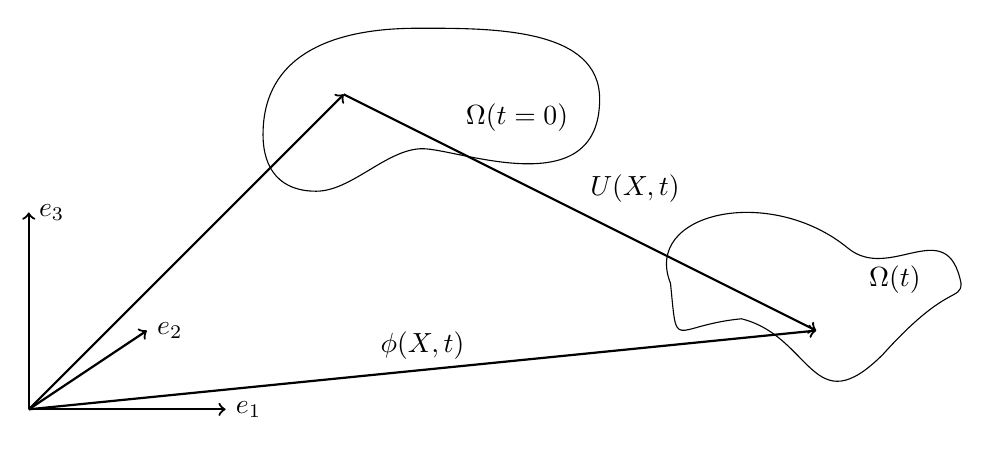
\begin{tikzpicture}
  %\draw[step=1.0,black,thin] (-3.,-1.) grid (3,4.);
  %\draw (-3,-1) -- (3,-1) -- (3,4) -- (-3,4) -- (-3,-1);
  \draw[thick,->] (-5,-2.5) -- (-2.5,-2.5) node [right] {$\vect{e}_1$};
  \draw[thick,->] (-5,-2.5) -- (-5,0.) node [right] {$\vect{e}_3$};
  \draw[thick,->] (-5,-2.5) -- (-3.5,-1.5) node [right] {$\vect{e}_2$};
  \begin{scope}[scale=0.45]
    \draw (-3,0.6) .. controls +(1,0) and +(-1,0) .. (0,1.8)  
    .. controls +(1,0) and +(0,-3) .. (5,3.2) 
    .. controls +(0,2) and +(2,0)  .. (0,5.2) 
    .. controls +(-1,0) and +(0,3) .. (-4.5,2.2) 
    .. controls +(0,-1) and +(-1,0).. (-3,0.6) ;
  \end{scope}
  \node at (1.2,1.2) {$\Omega(t=0)$};
  %% Deformed body +2.
  \begin{scope}[scale=0.9]
    \draw (0.+0.5+4.,0-1.5) ..controls (1.+0.5+4.,-0.25-1.5) and (1.+0.5+4.,-1.5-1.5) .. (2.+0.5+4.,-0.5-1.5) ..controls (2.9+0.5+4.,0.5-1.5) and (3.1+0.5+4.,0.25-1.5) .. (3.1+0.5+4.,0.5-1.5) ..controls (2.9+0.5+4.,1.5-1.5) and (2.1+0.5+4.,.5-1.5) .. (1.5+0.5+4.,1.-1.5) ..controls (0.4+0.5+4.,1.9-1.5) and (-1.4+0.5+4.,1.5-1.5) .. (-1.+0.5+4.,0.5-1.5)..controls (-0.4+0.+4.,-0.-2.) and (-1+0.5+4.,0.4-2.) .. (0+0.5+4.,0-1.5);
  \end{scope}
  \node at (6.,-0.85) {$\Omega(t)$};
  \draw[->,thick] (-5,-2.5) -- (-1.,1.5) node [midway,left] {$\X$};
  \draw[->,thick] (-5,-2.5) -- (5.,-1.5) node [midway,above] {$\vect{\phi}(\vect{X},t)$};
  \draw[->,thick] (-1.,1.5) -- (5.,-1.5) node [midway,above right] {$\vect{U}(\vect{X},t)$};
\end{tikzpicture}

%%% Local Variables:
%%% mode: latex
%%% TeX-master: "../../mainManuscript"
%%% End:
        \end{column}
        \begin{column}{0.5\textwidth}
          \begin{itemize}
          \item Reference mass density $\rho(\vect{X},t=0)=\rho_0(\vect{X})$
          \item Deformation gradient $\tens{F}(\vect{X},t)=\nablav_{\!0}\vect{\varphi}(\vect{X},t)$
          \item Cartesian coordinates system
          \end{itemize}
        \end{column}
      \end{columns}
    \end{block}
    \begin{block}{Balance equations \cite{Plohr}}
      \begin{equation*}
        \left.\begin{aligned}
            & \rho_0 \dot{\vect{v}} - \nablav_{\!0} \cdot \tens{\Pi} = \vect{0} \\
            & \dot{\tens{F}} - \nablav_{\!0} \cdot (\vect{v} \otimes \tens{I})= \tens{0}
          \end{aligned}\right\rbrace \Rightarrow \text{Conservative form: } \drond{\Ucb}{t} + \drond{\Fcb\cdot\vect{E}_\alpha}{X_\alpha} = \vect{0}
      \end{equation*}
      with $\Ucb = \matrice{\rho_0\vect{v} \\ \tens{F}} \: ; \: \Fcb\cdot\vect{E}_\alpha=\Fcb_\alpha=-\matrice{\tens{\Pi}\cdot\vect{E}_\alpha\\ \vect{v} \otimes\vect{E}_\alpha}$
    \end{block}
  \end{footnotesize}
  \footnoteCite{Plohr}
\end{frame}

\begin{frame}{Large deformations framework -- Constitutive equations}
  \begin{footnotesize}
    \begin{block}{Hyperelastic materials}
      %% Polyconvex, hyperbolicity ??
      From the thermodynamics: $\tens{\Pi}=\rho_0\drond{\psi}{\tens{F}}\: ; \: \dot{\tens{\Pi}}=\Hbb : \dot{\tens{F}}$ \\
      $\rho_0\psi$: Stored energy function, polyconvex $\Rightarrow$ hyperbolicity ensured \cite{Kluth}
    \end{block}
    \begin{block}{Quasi-linear form}
      Auxiliary vector $\Qcb$ \cite{Trangenstein91}: %$\Qcb=\matrice{\vect{v}\\\tens{\Pi}}$ 
      \begin{gather*}
        % \dot{\tens{\Pi}} = \Hbb(\tens{F}) : \dot{\tens{F}} \Rightarrow \text{Quasi-linear form: } \drond{\Qcb}{t} + \Absf^\alpha \drond{\Qcb}{X_\alpha} = \vect{0}
        \drond{\Ucb}{t} + \drond{\Fcb\cdot\vect{E}_\alpha}{X_\alpha} = \vect{0} \quad \Leftrightarrow \quad \drond{\Ucb}{\alert{\Qcb}}\drond{\alert{\Qcb}}{t} + \drond{\Fcb\cdot\vect{E}_\alpha}{\alert{\Qcb}}\drond{\alert{\Qcb}}{X_\alpha}=\vect{0} \\
        \drond{\Qcb}{t} + \Absf^\alpha \drond{\Qcb}{X_\alpha} = \vect{0}
      \end{gather*}
      where $\Qcb=\matrice{\vect{v}\\\tens{\Pi}} \: ; \: \Absf^\alpha = -\matrice{\tens{0}^2 & \frac{1}{\rho_0}\tens{I}\otimes\vect{E}_\alpha \\ \Hbb\cdot\vect{E}_\alpha & \tens{0}^4}$
    \end{block}
  \end{footnotesize}
  \footnoteCite{Kluth,Trangenstein91}
\end{frame}



\subsection{Discrete system}

\begin{frame}{Weak formulation}
  \begin{columns}
    \begin{column}{0.425\textwidth}
      \begin{block}{MPM space discretization}
        $N_p$ particles in $E$ elements
        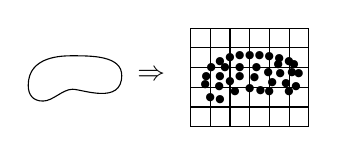
\begin{tikzpicture}[scale=0.25]
  % \draw[step=1.0,black,thin] (-3.,-1.) grid (3,4.);
  % \draw (-3,-1) -- (3,-1) -- (3,4) -- (-3,4) -- (-3,-1);
  \begin{scope}[scale=0.5]
    \draw (-3,0.6) .. controls +(1,0) and +(-1,0) .. (0,1.8)  
    .. controls +(1,0) and +(0,-3) .. (5,3.2) 
    .. controls +(0,2) and +(2,0)  .. (0,5.2) 
    .. controls +(-1,0) and +(0,3) .. (-4.5,2.2) 
    .. controls +(0,-1) and +(-1,0).. (-3,0.6) ;
    \begin{scope}  % pour limiter la portée du clip
      \clip (-3,0.6) .. controls +(1,0) and +(-1,0) .. (0,1.8) 
      .. controls +(1,0) and +(0,-3) .. (5,3.2)
      .. controls +(0,2) and +(2,0)  .. (0,5.2)
      .. controls +(-1,0) and +(0,3) .. (-4.5,2.2)
      .. controls +(0,-1) and +(-1,0).. (-3,0.6);
    \end{scope}
    %\node[below] at (0,1) {$\Omega$};
  \end{scope}
  \node at (4.,1.62) {$\Rightarrow$};
  \begin{scope}[shift={(9,0)}]
    \draw[step=1.0,black,thin] (-3.,-1.) grid (3,4.);
    % contour
    \node at (0,0.9) {\scriptsize$\bullet$}  ;
    \node at (2.5,1.65) {\scriptsize$\bullet$}  ; 
    \node at (0,2.6) {\scriptsize$\bullet$}  ;
    \node at (-2.25,1.1) {\scriptsize$\bullet$}  ; 
    \node at (-1.5,0.35) {\scriptsize$\bullet$}  ; 
    \node at (-2.,0.45) {\scriptsize$\bullet$} ;
    \node at (-2.2,1.5) {\scriptsize$\bullet$}  ; 
    \node at (-1.5,2.3) {\scriptsize$\bullet$} ; 
    \node at (2.35,1.) {\scriptsize$\bullet$}  ;
    \node at (2.25,2.15) {\scriptsize$\bullet$}  ;
    \node at (0.55,0.8) {\scriptsize$\bullet$}  ; 
    \node at (-0.5,2.6) {\scriptsize$\bullet$};
    \node at (0.5,2.59) {\scriptsize$\bullet$}  ;
    \node at (1.5,2.45) {\scriptsize$\bullet$}  ;
    \node at (1,0.75) {\scriptsize$\bullet$}; 
    \node at (2,0.75) {\scriptsize$\bullet$}  ;
    \node at (2,2.3) {\scriptsize$\bullet$}  ;
    \node at (1,2.55) {\scriptsize$\bullet$}  ;
    \node at (-1,2.5) {\scriptsize$\bullet$}  ; 
    \node at (-1.95,2.) {\scriptsize$\bullet$}  ;
    % interior
    \node at (-1.5,1.5) {\scriptsize$\bullet$}  ; 
    \node at (-1.25,2.) {\scriptsize$\bullet$}  ;
    \node at (-0.75,0.75) {\scriptsize$\bullet$}  ; 
    \node at (-1.55,1.){\scriptsize$\bullet$} ;
    \node at (-0.5,1.5) {\scriptsize$\bullet$}  ; 
    \node at (-0.5,2.) {\scriptsize$\bullet$}  ;
    \node at (0.25,1.45) {\scriptsize$\bullet$}  ;
    \node at (0.35,2.) {\scriptsize$\bullet$}  ;
    \node at (0.95,1.75) {\scriptsize$\bullet$}  ;
    \node at (1.15,1.2) {\scriptsize$\bullet$} ;
    \node at (1.45,2.15) {\scriptsize$\bullet$}  ; 
    \node at (1.55,1.65) {\scriptsize$\bullet$}  ;
    \node at (1.85,1.15) {\scriptsize$\bullet$}  ; 
    \node at (2.15,1.75) {\scriptsize$\bullet$}  ;
    \node at (-1.,1.25) {\scriptsize$\bullet$}  ;
    % \draw(3,0.5) -- (3.4,0.5) node [right]  {$\Omega_g$};
  \end{scope}
\end{tikzpicture}

%%% Local Variables:
%%% mode: latex
%%% TeX-master: "../presentation"
%%% End:

      \end{block}
    \end{column}
    \begin{column}{0.55\textwidth}
      \begin{block}{DG approximation \cite{DiPietro}}
        \vskip 14pt
        Broken polynomial space $\Vscr^k_h = \{\Vcb \in \Pscr^k(\Omega^e)\}$\\
        Approximate solution $\Ucb(\vect{X},t) \in \Vscr^k_h$ \\
        $\Vcb(\vect{X},t) = \sum_{i=1}^{N_{nodes}} S_i(\vect{X}) \Vcb^i(t)$
        \vskip 13pt
      \end{block}
    \end{column}
  \end{columns}
  \begin{block}{Element-wise weak form}
    \begin{equation*}
      \begin{aligned}
        & \text{Find $\Ucb\in \Vscr^1_h$ such that $\forall \:\Vcb,e,t \in \Vscr^1_h\times [1, E]\times \tau$:}\\
        & \int_{\Omega^e} \[\drond{\Ucb}{t} \Vcb - \Fcb_\alpha \drond{\Vcb}{X_\alpha}\]d\Omega + \int_{\partial \Omega^e} (\Fcb\cdot \vect{N}) d\Gamma = 0%\int_{\Omega^e} \Scb\Vcb d\Omega
      \end{aligned}
    \end{equation*}
  \end{block}
  \footnoteCite{DiPietro}
\end{frame}

\begin{frame}
  \begin{block}{Specific quantities}
    Approximation of the reference mass density \cite{Sulsky94}: $\rho_0(\vect{X})=\sum_{p=1}^{N_p}m_p \delta(\vect{X}^p-\vect{X})$ \\
    $\Rightarrow \: \Ucb = \rho_0 \bar{\Ucb} \:; \: \Fcb_\alpha = \rho_0 \bar{\Fcb}_\alpha$%\:; \: \Scb = \rho_0 \bar{\Scb}$
  \end{block}

  \begin{block}{Discrete weak form}
    \begin{equation*}
      \begin{aligned}
        & \text{Find $\Ucb\in \Vscr^1_h$ such that $\forall \:\Vcb,e,t \in \Vscr^1_h\times [1, E]\times \tau$:}\\
        & \sum_{p=1}^{N_p} m_p\[\ddroit{\bar{\Ucb}}{t} \Vcb - \bar{\Fcb}_\alpha \drond{\Vcb}{X_\alpha}\]_{\lvert_{\vect{X}=\vect{X}^p}} + \int_{\partial \Omega^e} (\Fcb\cdot \vect{N}) d\Gamma = \vect{0}
      \end{aligned}
    \end{equation*}
  \end{block}
  \footnoteCite{Sulsky94}
\end{frame}


\begin{frame}
  \begin{footnotesize}
    \begin{block}{Semi-discrete system}
      Introduction of polynomial approximation %$\Rightarrow  M_{ij} \ddroit{\bar{\Ucb}^j}{t}  - K_{ij}^\alpha \bar{\Fcb}^j_{\alpha} - \Scb^i + \hat{\Fcb}^i=  \vect{0} $
      \begin{equation*}
        M_{ij} \ddroit{\bar{\Ucb}^j}{t}  - K_{ij}^\alpha \bar{\Fcb}^j_{\alpha}  + \hat{\Fcb}^i=  \vect{0}
      \end{equation*}
      Diagonally lumped mass matrix $M^L_i=\sum_j M_{ij}$ \cite{Love}
    \end{block}
    \metroset{block=fill}
    \begin{block}{Explicit time discretization}
      \metroset{block=transparent}
      \begin{columns}
        \begin{column}{.4\textwidth}
          \begin{block}{\footnotesize Forward Euler}
            \vskip 7pt
            \begin{flalign*}
              M^L_i \frac{\bar{\Ucb}^{i,n+1} - \bar{\Ucb}^{i,n}}{\Delta t^n}=K_{ij}^\alpha \bar{\Fcb}^{j,n}_{\alpha}  - \hat{\Fcb}^{i,n}
            \end{flalign*}
            \vskip 14pt
          \end{block}
        \end{column}
        \begin{column}{.55\textwidth}
          \begin{block}{\footnotesize Second-order Runge-Kutta (RK2)}
            \vskip -5pt
            \begin{align*}
              & M^L_i \frac{\bar{\Ucb}^{i,n+1/2} - \bar{\Ucb}^{i,n}}{\Delta t^n}=\frac{1}{2}\(K_{ij}^\alpha \bar{\Fcb}^{j,n}_{\alpha}  - \hat{\Fcb}^{i,n}\) \\
              &M^L_i \frac{\bar{\Ucb}^{i,n+1} - \bar{\Ucb}^{i,n}}{\Delta t^n}=K_{ij}^\alpha \bar{\Fcb}^{j,n+1/2}_{\alpha}  - \hat{\Fcb}^{i,n+1/2}
            \end{align*}
          \end{block}
        \end{column}
      \end{columns}
    \end{block}
  \end{footnotesize}
  \footnoteCite{Love}
\end{frame}


\subsection{Interface fluxes}
\begin{frame}
  \begin{block}{Riemann problem}
    \begin{columns}
      \begin{column}{0.5\textwidth}
        \begin{footnotesize}
          \begin{align*}
          (\Rc\Pc): \quad &\drond{\Ucb}{t} + \drond{\Fcb_N}{\Ucb} \drond{\Ucb}{\xi }= \vect{0} \\ 
                          & \Ucb(\xi,0) = \left\lbrace 
                            \begin{aligned}
                              & \Ucb_L \: \text{if } \xi < 0 \\
                              & \Ucb_R \: \text{if } \xi > 0 
                            \end{aligned} \right.
          \end{align*}
        \end{footnotesize}
      \end{column}
      \begin{column}{0.3\textwidth}
        \begin{tikzpicture}[scale=0.5]
  \draw (10.,0.) -- (12.,6.) ; 
  \draw[fill=black] (9.85,0.1) circle (0.1) node [left] {$1$};	
  \draw[fill=black] (10.2,-0.0) circle (0.1) node [right] {$2$};	
  \draw[fill=black] (11.85,6.1) circle (0.1) node [left] {$4$};	
  \draw[fill=black] (12.2,6) circle (0.1) node [right] {$3$};	
  \draw[->,very thick] (11.,3.) -- (12,3 -1/3) node [right,below] {$X_N$}; 
  \node at (8,3.5) {$\vect{\Qc}_{L} = \frac{\vect{\Qc}_1 + \vect{\Qc}_4}{2}$}; \node at (14.5,3.5) {$\vect{\Qc}_{R} = \frac{\vect{\Qc}_2 + \vect{\Qc}_3}{2}$};
\end{tikzpicture}

      \end{column}
    \end{columns}
  \end{block}
  \vspace{-0.4cm}
  \begin{footnotesize}
    \begin{block}{Approximate Riemann solver \cite{Toro}}
      \begin{columns}
        \begin{column}{0.4\textwidth}
          \begin{itemize}
          \item Characteristic speeds $\lambda^i(\tens{F})$
          \item Simple waves
          \end{itemize}
        \end{column}  
        \begin{column}{0.55\textwidth}
          \begin{scriptsize}
  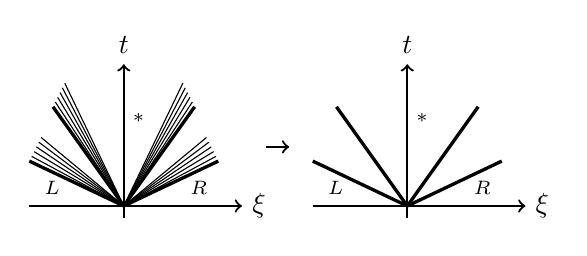
\begin{tikzpicture}[scale=0.3]
    \draw[->,thick] (-4,0) -- (5,0) node [right] {$\xi$};
    \draw[->,thick](0,-0.5) -- (0,6) node [above] {$t$};
    % Fastest left
    \draw[very thick](0,0) -- (-4,1.9) ;
    \draw(0,0) -- (-3.9,2.1) ;
    \draw(0,0) -- (-3.8,2.3) ;
    \draw(0,0) -- (-3.7,2.5) ;
    \draw(0,0) -- (-3.6,2.7) ;
    \draw(0,0) -- (-3.5,2.9) ;
    % Slowest left
    \draw[very thick](0,0) -- (-3.,4.2) ;
    \draw(0,0) -- (-2.9,4.4) ;
    \draw(0,0) -- (-2.8,4.6) ;
    \draw(0,0) -- (-2.7,4.8) ;
    \draw(0,0) -- (-2.6,5.0) ;
    \draw(0,0) -- (-2.5,5.2) ;
    % Fastest right
    \draw[very thick](0,0) -- (4,1.9) ;
    \draw(0,0) -- (3.9,2.1) ;
    \draw(0,0) -- (3.8,2.3) ;
    \draw(0,0) -- (3.7,2.5) ;
    \draw(0,0) -- (3.6,2.7) ;
    \draw(0,0) -- (3.5,2.9) ;
    % Slowest right
    \draw[very thick](0,0) -- (3.,4.2) ;
    \draw(0,0) -- (2.9,4.4) ;
    \draw(0,0) -- (2.8,4.6) ;
    \draw(0,0) -- (2.7,4.8) ;
    \draw(0,0) -- (2.6,5.0) ;
    \draw(0,0) -- (2.5,5.2) ;
    \node(a) at (-3,0.75) {$\Ucb_L$};
    \node(b) at (3.2,0.75) {$\Ucb_R$};
    \node(c) at (0.65,3.5) {$\Ucb^*$};
    \draw[->,thick](6.,2.5)--(7.,2.5) ;
    \begin{scope}[shift={(12.,0.)}]
      \draw[->,thick] (-4,0) -- (5,0) node [right] {$\xi$};
      \draw[->,thick](0,-0.5) -- (0,6) node [above] {$t$};
      % Fastest left
      \draw[very thick](0,0) -- (-4,1.9) ;
      % Slowest left
      \draw[very thick](0,0) -- (-3.,4.2) ;
      % Fastest right
      \draw[very thick](0,0) -- (4,1.9) ;
      % Slowest right
      \draw[very thick](0,0) -- (3.,4.2) ;
      \node(a) at (-3,0.75) {$\Ucb_L$};
      \node(b) at (3.2,0.75) {$\Ucb_R$};
      \node(c) at (0.65,3.5) {$\Ucb^*$};
    \end{scope}
  \end{tikzpicture}
\end{scriptsize}

%%% Local Variables:
%%% mode: latex
%%% TeX-master: "../../presentation"
%%% End:
        \end{column}
      \end{columns}
    \end{block}
    Computation of $\Ucb^* \Rightarrow$ corresponding flux: $\vect{\Fc}_N(\Ucb^*)$ \cite{Godunov_method}\\
    \alert{Integration of constitutive equations}
    
  \end{footnotesize}
  \vspace{-0.4cm}
  \footnoteCite{Toro,Godunov_method}
 \end{frame}

\begin{frame}%{\normalsize Boundary conditions}
  \begin{block}{\footnotesize Boundary Conditions: ghost nodes}
    \begin{columns}
      \begin{column}{0.3\textwidth}
        \begin{scriptsize}
  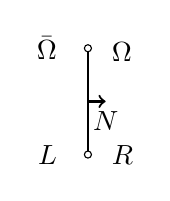
\begin{tikzpicture}[scale=0.45]
    \draw[thick] (0.0,0.0) -- (0,-3) ;
    \draw[->,thick] (0,-1.5) -- (0.5,-1.5) node [below] {$\vect{N}$};
    %\draw[->] (0,-1.5) -- (1,-1.5) node [below] {$\xi$};
    \node[left] at (-0.6,-3) {$L$};
    \node[right] at (.4,-3) {$R$};
    \node[left] at (-0.6,0) {$\bar{\Omega}$};
    \node[right] at (.4,-0.1) {$\Omega$};
    \draw [fill=white] (0,0) circle (0.1);
    \draw [fill=white] (0,-3) circle (0.1);
  \end{tikzpicture}	
\end{scriptsize}

%%% Local Variables:
%%% mode: latex
%%% TeX-master: "../../presentation"
%%% End:
      \end{column}
      \begin{column}{0.6\textwidth}
        \begin{scriptsize}
          \begin{itemize}
          \item[] Enforce $\Ucb_L$ such that $\Ucb^*=\Ucb^{imp}$
          \item[] Problem: apply strain rather than stress 
          \end{itemize}
        \end{scriptsize}
      \end{column}	
    \end{columns}
  \end{block}
  \begin{scriptsize}
  $\Rightarrow $ Quasi-linear form with suitable $\Qcb$ (\textit{i.e. containing stress})\\
  \alert{Also avoid the integration of constitutive equations at element interfaces !}
  \end{scriptsize}
  \begin{block}{\footnotesize Transverse corrections: Adaptation of the Corner Transport Upwind method \cite{Colella_CTU}}
    \centering
    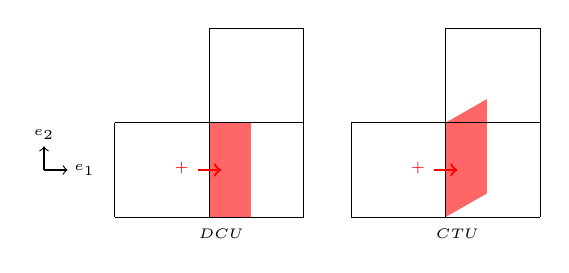
\begin{tikzpicture}[scale=0.6]
  \fill[Red!60] (0,0) rectangle (.875,-2);
  \draw (-2,0) -- (2,0.);\draw (0.,2) -- (0,-2.);\draw (0,2) -- (2,2);
  \draw (-2.,-2.) -- (2.,-2.);\draw (2,2.) -- (2,-2.);\draw (-2,-2) -- (-2,0);
  \begin{tiny}
    \draw[->,thick,Red] (-.25,-1.) node [left] {$\Ac^+$} -- (.25,-1.) ;
    \draw[->] (-3.5,-1.) -- (-3,-1.) node[right] {$\vect{e}_1$};
    \draw[->] (-3.5,-1.) -- (-3.5,-0.5) node[above] {$\vect{e}_2$};
    \node at (0.25,-2.35) {$DCU$};
  \end{tiny}
  \begin{scope}[shift={(5.,0.)}]
    \fill[Red!60] (0,0) rectangle (.875,-2);
    \fill[Red!60] (0,0) -- (.875,0) -- (.875,.5) -- (0.,0.); %% Red triangle
    \fill[white] (0,0-2) -- (.875,0-2) -- (.875,.5-2) -- (0.,0.-2); %% White triangle
    \draw (-2,0) -- (2,0.);\draw (0.,2) -- (0,-2.);\draw (0,2) -- (2,2);
    \draw (-2.,-2.) -- (2.,-2.);\draw (2,2.) -- (2,-2.);\draw (-2,-2) -- (-2,0);
    \begin{tiny}
      \draw[->,thick,Red] (-.25,-1.) node [left] {$\Ac^+$} -- (.25,-1.) ;
      \node at (0.25,-2.35) {$CTU$};
    \end{tiny}    
  \end{scope}
\end{tikzpicture}

%%% Local Variables:
%%% mode: latex
%%% TeX-master: "../../presentation"
%%% End:

  \end{block}
  \footnoteCite{Colella_CTU}
\end{frame}

\subsection{Solution scheme}
%\begin{frame}{Procedure between $t^n$ and $t^n + \Delta t^n=t^{n+1}$}
  \begin{footnotesize}
    \begin{overprint}
      %% Computation of matrices
      \onslide<1>
      \begin{equation*}
        \text{Discrete system: }\alert{M^L_{i}} \frac{\bar{\Ucb}^{i,n+1} - \bar{\Ucb}^{i,n}}{\Delta t^n}  - \alert{K_{ij}^\alpha} \bar{\Fcb}^{j,n}_{\alpha}  + \hat{\Fcb}^{i,n}=  \vect{0}
      \end{equation*}
      \begin{columns}
        \begin{column}{0.4\textwidth}
          \begin{itemize}
          \item[(1)] Computation of matrices $M_i^L$ and $K_{ij}^\alpha$
          \end{itemize}
        \end{column}
        \vrule{}
        \begin{column}{0.6\textwidth}
          \begin{block}{Computation of matrices $M_i^L$ and $K_{ij}^\alpha$}
            \begin{columns}
              \begin{column}{0.3\textwidth}
                \vskip 0.9pt
                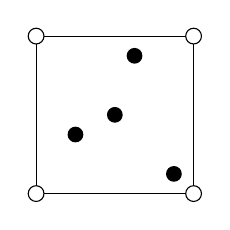
\begin{tikzpicture}
                  \draw (0,0) rectangle (2,2);
                  \fill[white] (0,0) circle (0.1); \fill[white] (0,2) circle (0.1); \fill[white] (2,0) circle (0.1); \fill[white] (2,2) circle (0.1);
                  \draw (0,0) circle (0.1); \draw (0,2) circle (0.1); \draw (2,0) circle (0.1); \draw (2,2) circle (0.1);
                  \fill[black] (0.5,0.75) circle (0.1); \fill[black] (1.25,1.75) circle (0.1); \fill[black] (1.75,0.25) circle (0.1); \fill[black] (1,1) circle (0.1);
                \end{tikzpicture}
              \end{column}
              \begin{column}{0.6\textwidth}
                States of particles known at time $t^n$:
                \begin{equation*}
                  \left\lbrace\begin{aligned}
                      & \vect{v}^{p,n},\tens{F}^{p,n},\tens{\Pi}^{p,n} \: \rightarrow \:\Ucb^{p,n},\Qcb^{p,n}\\
                      & \vect{X}^{p,n} \: \rightarrow \:M_i^{L,n},K_{ij}^{\alpha,n}
                    \end{aligned}\right.
                \end{equation*}
                
              \end{column}
            \end{columns}
          \end{block}
        \end{column}
      \end{columns}

      %% Particles -> Nodes
      \onslide<2>
      \begin{equation*}
        \text{Discrete system: }M^L_{i} \frac{\bar{\Ucb}^{i,n+1} - \alert{\bar{\Ucb}^{i,n}}}{\Delta t^n}  - K_{ij}^\alpha \bar{\Fcb}^{j,n}_{\alpha}  + \hat{\Fcb}^{i,n}=  \vect{0}
      \end{equation*}
      \begin{columns}
        \begin{column}{0.4\textwidth}
          \begin{itemize}
          \item[(1)] Computation of matrices $M_i^L$ and $K_{ij}^\alpha$
          \item[(2)] Projection particles $\rightarrow$ nodes
          \end{itemize}
        \end{column}
        \vrule{}
        \begin{column}{0.6\textwidth}
          \begin{block}{Projection particles $\rightarrow$ nodes}
            \begin{columns}
              \begin{column}{0.3\textwidth}
                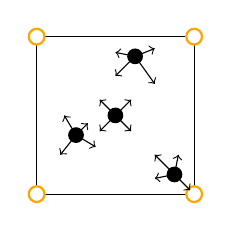
\begin{tikzpicture}
                  \draw (0,0) rectangle (2,2);
                  \fill[white] (0,0) circle (0.1); \fill[white] (0,2) circle (0.1); \fill[white] (2,0) circle (0.1); \fill[white] (2,2) circle (0.1);
                  \draw[Orange,thick] (0,0) circle (0.1); \draw[Orange,thick] (0,2) circle (0.1); \draw[Orange,thick] (2,0) circle (0.1); \draw[Orange,thick] (2,2) circle (0.1);
                  \fill[black] (0.5,0.75) circle (0.1); \fill[black] (1.25,1.75) circle (0.1); \fill[black] (1.75,0.25) circle (0.1); \fill[black] (1,1) circle (0.1);
                  %% North arrows
                  \draw[->,black] (1.25,1.75) -- (1.5,1.85);\draw[->,black] (1.25,1.75) -- (1.,1.8);\draw[->,black] (1.25,1.75) -- (1.,1.5);\draw[->,black] (1.25,1.75) -- (1.5,1.4);
                  %% West arrows
                  \draw[->,black] (0.5,0.75) -- (0.3,0.5);\draw[->,black] (0.5,0.75) -- (0.35,1.);\draw[->,black] (0.5,0.75) -- (0.75,.6);\draw[->,black] (0.5,0.75) -- (.65,0.9);
                  %% Center arrows
                  \draw[->,black] (1,1) -- (1.2,1.2);\draw[->,black] (1,1) -- (1.2,0.8);\draw[->,black] (1,1) -- (0.8,1.2);\draw[->,black] (1,1) -- (0.8,0.8);
                  %% South arrows
                  \draw[->,black] (1.75,0.25) -- (1.95,.05);\draw[->,black] (1.75,0.25) -- (1.8,.5);\draw[->,black] (1.75,0.25) -- (1.5,.5);\draw[->,black] (1.75,0.25) -- (1.5,0.2);
                \end{tikzpicture}
              \end{column}
              \begin{column}{0.6\textwidth}
                \begin{equation*}
                  \begin{aligned}
                    & M^{L,n}_i \alert{\bar{\Ucb}^{i,n}} = \sum_{p=1}^{N_p} m_p \bar{\Ucb}^{p,n}\\
                    & M^{L,n}_i \alert{\Qcb^{i,n}} = \sum_{p=1}^{N_p} m_p \Qcb^{p,n}
                  \end{aligned}
                \end{equation*}
              \end{column}
            \end{columns}
          \end{block}
        \end{column}
      \end{columns}
      
      %% Computation of numerical fluxes (volume + intercell)
      \onslide<3>
      \begin{equation*}
        \text{Discrete system: }M^L_{i} \frac{\bar{\Ucb}^{i,n+1} - \bar{\Ucb}^{i,n}}{\Delta t^n}  - K_{ij}^\alpha \alert{\bar{\Fcb}^{j,n}_{\alpha}}  + \alert{\hat{\Fcb}^{i,n}}=  \vect{0}
      \end{equation*}
      \begin{columns}
        \begin{column}{0.4\textwidth}
          \begin{itemize}
          \item[(1)] Computation of matrices $M_i^L$ and $K_{ij}^\alpha$
          \item[(2)] Projection particles $\rightarrow$ nodes
          \item[(3)] Computation of fluxes
          \end{itemize}
        \end{column}
        \vrule{}
        \begin{column}{0.6\textwidth}
          \begin{block}{Computation of fluxes}
            \begin{columns}
              \begin{column}{0.4\textwidth}
                \begin{block}{\footnotesize Volume fluxes}
                  $\bar{\Ucb}^{i,n},\Qcb^{i,n} \rightarrow \bar{\Fcb}^{i,n}_\alpha$
                \end{block}
              \end{column}
              \begin{column}{0.55\textwidth}
                \begin{block}{\footnotesize Intercell fluxes}
                  Approximate Riemann solver $\rightarrow \hat{\Fcb}^i$
                \end{block}
              \end{column}
            \end{columns}
          \end{block}
        \end{column}
      \end{columns}
      
      %% Time integration + Interpolation
      \onslide<4>
      \begin{equation*}
        \text{Discrete system: }M^L_{i} \frac{\alert{\bar{\Ucb}^{i,n+1}} - \bar{\Ucb}^{i,n}}{\Delta t^n}  - K_{ij}^\alpha \bar{\Fcb}^{j,n}_{\alpha}  + \hat{\Fcb}^{i,n}=  \vect{0}
      \end{equation*}
      \begin{columns}
        \begin{column}{0.4\textwidth}
          \begin{itemize}
          \item[(1)] Computation of matrices $M_i^L$ and $K_{ij}^\alpha$
          \item[(2)] Projection particles $\rightarrow$ nodes
          \item[(3)] Computation of fluxes
          \item[(4)] Explicit time integration; Interpolation
          \end{itemize}
        \end{column}
        \vrule{}
        \begin{column}{0.6\textwidth}
          \begin{block}{Explicit time integration; Interpolation}
            
            \begin{columns}
              \begin{column}{0.4\textwidth}
                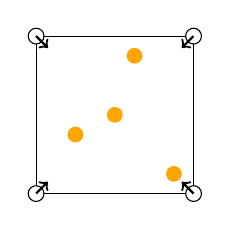
\begin{tikzpicture}
                  \draw (0,0) rectangle (2,2);
                  \fill[white] (0,0) circle (0.1); \fill[white] (0,2) circle (0.1); \fill[white] (2,0) circle (0.1); \fill[white] (2,2) circle (0.1);
                  \draw (0,0) circle (0.1); \draw (0,2) circle (0.1); \draw (2,0) circle (0.1); \draw (2,2) circle (0.1);
                  \draw[->,thick] (0,0) -- (0.15,0.15);
                  \draw[->,thick] (2,0) -- (1.85,0.15);
                  \draw[->,thick] (2,2) -- (1.85,1.85);
                  \draw[->,thick] (0,2) -- (.15,1.85);
                  
                  \fill[Orange] (0.5,0.75) circle (0.1); \fill[Orange] (1.25,1.75) circle (0.1); \fill[Orange] (1.75,0.25) circle (0.1); \fill[Orange] (1,1) circle (0.1);
                  
                  % \fill[black!50] (0.5,0.75) circle (0.1); \fill[black!50] (1.25,1.75) circle (0.1); \fill[black!50] (1.75,0.25) circle (0.1); \fill[black!50] (1,1) circle (0.1);
                  % \fill[black] (0.75,1.25) circle (0.1); \fill[black] (1.75,2.25) circle (0.1); \fill[black] (2.1,0.75) circle (0.1); \fill[black] (1.5,1.5) circle (0.1);
                  % \path[->,thick,black] (0.5,0.75) edge[bend left] (0.73,1.22);
                  % \path[->,thick,black] (1.25,1.75) edge[bend right] (1.75,2.21);
                  % \path[->,thick,black](1.75,0.25) edge[bend left] (2.,0.75);
                  % \path[->,thick,black](1,1) edge[bend right] (1.5,1.4);
                \end{tikzpicture}
              \end{column}
              \begin{column}{0.55\textwidth}
                \begin{equation*}
                  \alert{\bar{\Ucb}^{p,n+1}}=\sum_{i=1}^{N_{nodes}} S_{i}(\vect{X}^{p}) \bar{\Ucb}^{i,n+1}
                \end{equation*}
              \end{column}
            \end{columns}
          \end{block}
        \end{column}
      \end{columns}
           
      %% Kinematic and constitutive updates
      \onslide<5>
      \begin{columns}
        \begin{column}{0.4\textwidth}
          \begin{itemize}
          \item[(1)] Computation of matrices $M_i^L$ and $K_{ij}^\alpha$
          \item[(2)] Projection particles $\rightarrow$ nodes
          \item[(3)] Computation of fluxes
          \item[(4)] Explicit time integration; Interpolation
          \item[(5)] Kinematics and constitutive updates
          \end{itemize}
        \end{column}
        \vrule{}
        \begin{column}{0.6\textwidth}
          \begin{block}{Kinematics and constitutive updates}
            \begin{columns}
              \begin{column}{0.4\textwidth}
                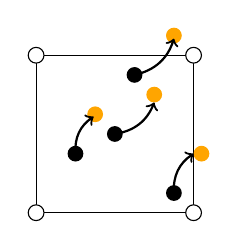
\begin{tikzpicture}
                  \draw (0,0) rectangle (2,2);
                  \fill[white] (0,0) circle (0.1); \fill[white] (0,2) circle (0.1); \fill[white] (2,0) circle (0.1); \fill[white] (2,2) circle (0.1);
                  \draw (0,0) circle (0.1); \draw (0,2) circle (0.1); \draw (2,0) circle (0.1); \draw (2,2) circle (0.1);
                  \fill[black] (0.5,0.75) circle (0.1); \fill[black] (1.25,1.75) circle (0.1); \fill[black] (1.75,0.25) circle (0.1); \fill[black] (1,1) circle (0.1);
                  \fill[Orange] (0.75,1.25) circle (0.1); \fill[Orange] (1.75,2.25) circle (0.1); \fill[Orange] (2.1,0.75) circle (0.1); \fill[Orange] (1.5,1.5) circle (0.1);
                  \path[->,thick,black] (0.5,0.75) edge[bend left] (0.73,1.22);
                  \path[->,thick,black] (1.25,1.75) edge[bend right] (1.75,2.21);
                  \path[->,thick,black](1.75,0.25) edge[bend left] (2.,0.75);
                  \path[->,thick,black](1,1) edge[bend right] (1.5,1.4);
                \end{tikzpicture}
              \end{column}
              \begin{column}{0.55\textwidth}
                \begin{flalign*}
                  \begin{aligned}
                    & \alert{\tens{\Pi}^{p,n+1}}=g(\tens{F}^{p,n+1})\\
                    & \alert{\vect{\varphi}^{p,n+1}}= \vect{\varphi}^{p,n} +\Delta t^n \vect{v}^{p,n+1}
                  \end{aligned}
                \end{flalign*}
              \end{column}
            \end{columns}
          \end{block}
        \end{column}
      \end{columns}
      
      
      %% Rebuild the grid if needed
      \onslide<6>
      \begin{columns}
        \begin{column}{0.4\textwidth}
          \begin{itemize}
          \item[(1)] Computation of matrices $M_i^L$ and $K_{ij}^\alpha$
          \item[(2)] Projection particles $\rightarrow$ nodes
          \item[(3)] Computation of fluxes
          \item[(4)] Explicit time integration; Interpolation
          \item[(5)] Kinematics and constitutive updates
          \item[(6)] Reconstruction of the grid (if needed) 
          \end{itemize}
        \end{column}
        \vrule{}
        \begin{column}{0.6\textwidth}
          \begin{block}{Reconstruction of the grid (if needed)}
            \begin{columns}
              \begin{column}{0.4\textwidth}
                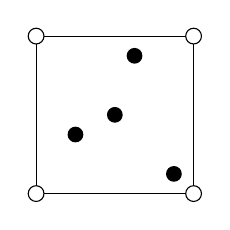
\begin{tikzpicture}
                  \draw (0,0) rectangle (2,2);
                  \fill[white] (0,0) circle (0.1); \fill[white] (0,2) circle (0.1); \fill[white] (2,0) circle (0.1); \fill[white] (2,2) circle (0.1);
                  \draw (0,0) circle (0.1); \draw (0,2) circle (0.1); \draw (2,0) circle (0.1); \draw (2,2) circle (0.1);
                  \fill[black] (0.5,0.75) circle (0.1); \fill[black] (1.25,1.75) circle (0.1); \fill[black] (1.75,0.25) circle (0.1); \fill[black] (1,1) circle (0.1);
                \end{tikzpicture}
              \end{column}
              \begin{column}{0.55\textwidth}
                \centering
                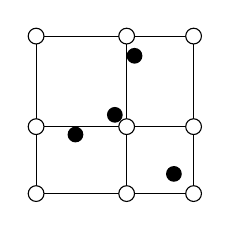
\begin{tikzpicture}
                  \draw (0,0) rectangle (2.,2.);
                  \draw (1.15,0.85) rectangle (2.,0);
                  \draw (1.15,0.85) rectangle (2.,2);
                  \draw (1.15,0.85) rectangle (0.,2);
                  %% Old nodes
                  \fill[white] (0,0) circle (0.1);
                  \fill[white] (0,2) circle (0.1);
                  \fill[white] (2,0) circle (0.1);
                  \fill[white] (2,2) circle (0.1);
                  \draw (0,0) circle (0.1);
                  \draw (0,2) circle (0.1);
                  \draw (2,0) circle (0.1);
                  \draw (2,2) circle (0.1);

                  %% Added nodes
                  \fill[white] (1.15,0.85) circle (0.1);
                  \fill[white] (0,0.85) circle (0.1);
                  \fill[white] (2,0.85) circle (0.1);
                  \fill[white] (1.15,0) circle (0.1);
                  \fill[white] (1.15,2) circle (0.1);
                  \draw (1.15,0.85) circle (0.1);
                  \draw (0,0.85) circle (0.1);
                  \draw (2,0.85) circle (0.1);
                  \draw (1.15,0) circle (0.1);
                  \draw (1.15,2) circle (0.1);

                  %% Particles
                  \fill[black] (0.5,0.75) circle (0.1); \fill[black] (1.25,1.75) circle (0.1); \fill[black] (1.75,0.25) circle (0.1); \fill[black] (1,1) circle (0.1);
                \end{tikzpicture}
              \end{column}
            \end{columns}
          \end{block}
        \end{column}
      \end{columns}
    \end{overprint}
  \end{footnotesize}
\end{frame}

\begin{frame}{Procedure between $t^n$ and $t^n + \Delta t^n=t^{n+1}$}
  \begin{footnotesize}
    %% Computation of matrices
    \begin{equation*}
      \text{Discrete system: }\alert{M^L_{i}} \frac{\bar{\Ucb}^{i,n+1} - \bar{\Ucb}^{i,n}}{\Delta t^n}  - \alert{K_{ij}^\alpha} \bar{\Fcb}^{j,n}_{\alpha}  + \hat{\Fcb}^{i,n}=  \vect{0}
    \end{equation*}
    \begin{columns}
      \begin{column}{0.4\textwidth}
        \begin{itemize}
        \item[(1)] Computation of matrices $M_i^L$ and $K_{ij}^\alpha$
        \end{itemize}
      \end{column}
      \vrule{}
      \begin{column}{0.6\textwidth}
        \begin{block}{Computation of matrices $M_i^L$ and $K_{ij}^\alpha$}
          \begin{columns}
            \begin{column}{0.3\textwidth}
              \vskip 0.9pt
              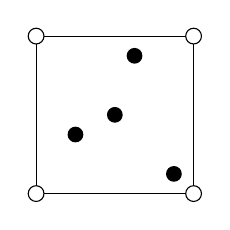
\begin{tikzpicture}
                \draw (0,0) rectangle (2,2);
                \fill[white] (0,0) circle (0.1); \fill[white] (0,2) circle (0.1); \fill[white] (2,0) circle (0.1); \fill[white] (2,2) circle (0.1);
                \draw (0,0) circle (0.1); \draw (0,2) circle (0.1); \draw (2,0) circle (0.1); \draw (2,2) circle (0.1);
                \fill[black] (0.5,0.75) circle (0.1); \fill[black] (1.25,1.75) circle (0.1); \fill[black] (1.75,0.25) circle (0.1); \fill[black] (1,1) circle (0.1);
              \end{tikzpicture}
            \end{column}
            \begin{column}{0.6\textwidth}
              States of particles known at time $t^n$:
              \begin{equation*}
                \left\lbrace\begin{aligned}
                    & \vect{v}^{p,n},\tens{F}^{p,n},\tens{\Pi}^{p,n} \: \rightarrow \:\Ucb^{p,n},\Qcb^{p,n}\\
                    & \vect{X}^{p,n} \: \rightarrow \:M_i^{L,n},K_{ij}^{\alpha,n}
                  \end{aligned}\right.
              \end{equation*}
              
            \end{column}
          \end{columns}
        \end{block}
      \end{column}
    \end{columns}
  \end{footnotesize}
\end{frame}

\begin{frame}{Procedure between $t^n$ and $t^n + \Delta t^n=t^{n+1}$}
  \begin{footnotesize}
    %% Particles -> Nodes
    \begin{equation*}
      \text{Discrete system: }M^L_{i} \frac{\bar{\Ucb}^{i,n+1} - \alert{\bar{\Ucb}^{i,n}}}{\Delta t^n}  - K_{ij}^\alpha \bar{\Fcb}^{j,n}_{\alpha}  + \hat{\Fcb}^{i,n}=  \vect{0}
    \end{equation*}
    \begin{columns}
      \begin{column}{0.4\textwidth}
        \begin{itemize}
        \item[(1)] Computation of matrices $M_i^L$ and $K_{ij}^\alpha$
        \item[(2)] Projection particles $\rightarrow$ nodes
        \end{itemize}
      \end{column}
      \vrule{}
      \begin{column}{0.6\textwidth}
        \begin{block}{Projection particles $\rightarrow$ nodes}
          \begin{columns}
            \begin{column}{0.3\textwidth}
              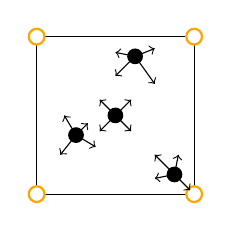
\begin{tikzpicture}
                \draw (0,0) rectangle (2,2);
                \fill[white] (0,0) circle (0.1); \fill[white] (0,2) circle (0.1); \fill[white] (2,0) circle (0.1); \fill[white] (2,2) circle (0.1);
                \draw[Orange,thick] (0,0) circle (0.1); \draw[Orange,thick] (0,2) circle (0.1); \draw[Orange,thick] (2,0) circle (0.1); \draw[Orange,thick] (2,2) circle (0.1);
                \fill[black] (0.5,0.75) circle (0.1); \fill[black] (1.25,1.75) circle (0.1); \fill[black] (1.75,0.25) circle (0.1); \fill[black] (1,1) circle (0.1);
                %% North arrows
                \draw[->,black] (1.25,1.75) -- (1.5,1.85);\draw[->,black] (1.25,1.75) -- (1.,1.8);\draw[->,black] (1.25,1.75) -- (1.,1.5);\draw[->,black] (1.25,1.75) -- (1.5,1.4);
                %% West arrows
                \draw[->,black] (0.5,0.75) -- (0.3,0.5);\draw[->,black] (0.5,0.75) -- (0.35,1.);\draw[->,black] (0.5,0.75) -- (0.75,.6);\draw[->,black] (0.5,0.75) -- (.65,0.9);
                %% Center arrows
                \draw[->,black] (1,1) -- (1.2,1.2);\draw[->,black] (1,1) -- (1.2,0.8);\draw[->,black] (1,1) -- (0.8,1.2);\draw[->,black] (1,1) -- (0.8,0.8);
                %% South arrows
                \draw[->,black] (1.75,0.25) -- (1.95,.05);\draw[->,black] (1.75,0.25) -- (1.8,.5);\draw[->,black] (1.75,0.25) -- (1.5,.5);\draw[->,black] (1.75,0.25) -- (1.5,0.2);
              \end{tikzpicture}
            \end{column}
            \begin{column}{0.6\textwidth}
              \begin{equation*}
                \begin{aligned}
                  & M^{L,n}_i \alert{\bar{\Ucb}^{i,n}} = \sum_{p=1}^{N_p} m_p \bar{\Ucb}^{p,n}\\
                  & M^{L,n}_i \alert{\Qcb^{i,n}} = \sum_{p=1}^{N_p} m_p \Qcb^{p,n}
                \end{aligned}
              \end{equation*}
            \end{column}
          \end{columns}
        \end{block}
      \end{column}
    \end{columns}
  \end{footnotesize}
\end{frame}


\begin{frame}{Procedure between $t^n$ and $t^n + \Delta t^n=t^{n+1}$}
  \begin{footnotesize}
    %% Computation of numerical fluxes (volume + intercell)
    \begin{equation*}
      \text{Discrete system: }M^L_{i} \frac{\bar{\Ucb}^{i,n+1} - \bar{\Ucb}^{i,n}}{\Delta t^n}  - K_{ij}^\alpha \alert{\bar{\Fcb}^{j,n}_{\alpha}}  + \alert{\hat{\Fcb}^{i,n}}=  \vect{0}
    \end{equation*}
    \begin{columns}
      \begin{column}{0.4\textwidth}
        \begin{itemize}
        \item[(1)] Computation of matrices $M_i^L$ and $K_{ij}^\alpha$
        \item[(2)] Projection particles $\rightarrow$ nodes
        \item[(3)] Computation of fluxes
        \end{itemize}
      \end{column}
      \vrule{}
      \begin{column}{0.6\textwidth}
        \begin{block}{Computation of fluxes}
          \begin{columns}
            \begin{column}{0.4\textwidth}
              \begin{block}{\footnotesize Volume fluxes}
                $\bar{\Ucb}^{i,n},\Qcb^{i,n} \rightarrow \bar{\Fcb}^{i,n}_\alpha$
              \end{block}
            \end{column}
            \begin{column}{0.55\textwidth}
              \begin{block}{\footnotesize Intercell fluxes}
                Approximate Riemann solver $\rightarrow \hat{\Fcb}^i$
              \end{block}
            \end{column}
          \end{columns}
        \end{block}
      \end{column}
    \end{columns}
  \end{footnotesize}
\end{frame}

\begin{frame}{Procedure between $t^n$ and $t^n + \Delta t^n=t^{n+1}$}
  \begin{footnotesize}
    %% Time integration + Interpolation
    \begin{equation*}
      \text{Discrete system: }M^L_{i} \frac{\alert{\bar{\Ucb}^{i,n+1}} - \bar{\Ucb}^{i,n}}{\Delta t^n}  - K_{ij}^\alpha \bar{\Fcb}^{j,n}_{\alpha}  + \hat{\Fcb}^{i,n}=  \vect{0}
    \end{equation*}
    \begin{columns}
      \begin{column}{0.4\textwidth}
        \begin{itemize}
        \item[(1)] Computation of matrices $M_i^L$ and $K_{ij}^\alpha$
        \item[(2)] Projection particles $\rightarrow$ nodes
        \item[(3)] Computation of fluxes
        \item[(4)] Explicit time integration; Interpolation
        \end{itemize}
      \end{column}
      \vrule{}
      \begin{column}{0.6\textwidth}
        \begin{block}{Explicit time integration; Interpolation}
          
          \begin{columns}
            \begin{column}{0.4\textwidth}
              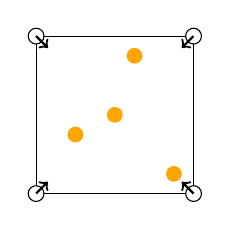
\begin{tikzpicture}
                \draw (0,0) rectangle (2,2);
                \fill[white] (0,0) circle (0.1); \fill[white] (0,2) circle (0.1); \fill[white] (2,0) circle (0.1); \fill[white] (2,2) circle (0.1);
                \draw (0,0) circle (0.1); \draw (0,2) circle (0.1); \draw (2,0) circle (0.1); \draw (2,2) circle (0.1);
                \draw[->,thick] (0,0) -- (0.15,0.15);
                \draw[->,thick] (2,0) -- (1.85,0.15);
                \draw[->,thick] (2,2) -- (1.85,1.85);
                \draw[->,thick] (0,2) -- (.15,1.85);
                
                \fill[Orange] (0.5,0.75) circle (0.1); \fill[Orange] (1.25,1.75) circle (0.1); \fill[Orange] (1.75,0.25) circle (0.1); \fill[Orange] (1,1) circle (0.1);
              \end{tikzpicture}
            \end{column}
            \begin{column}{0.55\textwidth}
              \begin{equation*}
                \alert{\bar{\Ucb}^{p,n+1}}=\sum_{i=1}^{N_{nodes}} S_{i}(\vect{X}^{p}) \bar{\Ucb}^{i,n+1}
              \end{equation*}
            \end{column}
          \end{columns}
        \end{block}
      \end{column}
    \end{columns}
  \end{footnotesize}
\end{frame}

\begin{frame}{Procedure between $t^n$ and $t^n + \Delta t^n=t^{n+1}$}
  \begin{footnotesize}
    %% Kinematic and constitutive updates
    \begin{columns}
      \begin{column}{0.4\textwidth}
        \begin{itemize}
        \item[(1)] Computation of matrices $M_i^L$ and $K_{ij}^\alpha$
        \item[(2)] Projection particles $\rightarrow$ nodes
        \item[(3)] Computation of fluxes
        \item[(4)] Explicit time integration; Interpolation
        \item[(5)] Kinematics and constitutive updates
        \end{itemize}
      \end{column}
      \vrule{}
      \begin{column}{0.6\textwidth}
        \begin{block}{Kinematics and constitutive updates}
          \begin{columns}
            \begin{column}{0.4\textwidth}
              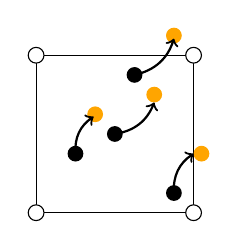
\begin{tikzpicture}
                \draw (0,0) rectangle (2,2);
                \fill[white] (0,0) circle (0.1); \fill[white] (0,2) circle (0.1); \fill[white] (2,0) circle (0.1); \fill[white] (2,2) circle (0.1);
                \draw (0,0) circle (0.1); \draw (0,2) circle (0.1); \draw (2,0) circle (0.1); \draw (2,2) circle (0.1);
                \fill[black] (0.5,0.75) circle (0.1); \fill[black] (1.25,1.75) circle (0.1); \fill[black] (1.75,0.25) circle (0.1); \fill[black] (1,1) circle (0.1);
                \fill[Orange] (0.75,1.25) circle (0.1); \fill[Orange] (1.75,2.25) circle (0.1); \fill[Orange] (2.1,0.75) circle (0.1); \fill[Orange] (1.5,1.5) circle (0.1);
                \path[->,thick,black] (0.5,0.75) edge[bend left] (0.73,1.22);
                \path[->,thick,black] (1.25,1.75) edge[bend right] (1.75,2.21);
                \path[->,thick,black](1.75,0.25) edge[bend left] (2.,0.75);
                \path[->,thick,black](1,1) edge[bend right] (1.5,1.4);
              \end{tikzpicture}
            \end{column}
            \begin{column}{0.55\textwidth}
              \begin{flalign*}
                \begin{aligned}
                  & \alert{\tens{\Pi}^{p,n+1}}=g(\tens{F}^{p,n+1})\\
                  & \alert{\vect{\varphi}^{p,n+1}}= \vect{\varphi}^{p,n} +\Delta t^n \vect{v}^{p,n+1}
                \end{aligned}
              \end{flalign*}
            \end{column}
          \end{columns}
        \end{block}
      \end{column}
    \end{columns}
  \end{footnotesize}
\end{frame}
      
\begin{frame}{Procedure between $t^n$ and $t^n + \Delta t^n=t^{n+1}$}
  \begin{footnotesize}
    %% Rebuild the grid if needed
    \begin{columns}
      \begin{column}{0.4\textwidth}
        \begin{itemize}
        \item[(1)] Computation of matrices $M_i^L$ and $K_{ij}^\alpha$
        \item[(2)] Projection particles $\rightarrow$ nodes
        \item[(3)] Computation of fluxes
        \item[(4)] Explicit time integration; Interpolation
        \item[(5)] Kinematics and constitutive updates
        \item[(6)] Reconstruction of the grid (if needed) 
        \end{itemize}
      \end{column}
      \vrule{}
      \begin{column}{0.6\textwidth}
        \begin{block}{Reconstruction of the grid (if needed)}
          \begin{columns}
            \begin{column}{0.4\textwidth}
              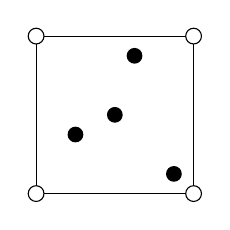
\begin{tikzpicture}
                \draw (0,0) rectangle (2,2);
                \fill[white] (0,0) circle (0.1); \fill[white] (0,2) circle (0.1); \fill[white] (2,0) circle (0.1); \fill[white] (2,2) circle (0.1);
                \draw (0,0) circle (0.1); \draw (0,2) circle (0.1); \draw (2,0) circle (0.1); \draw (2,2) circle (0.1);
                \fill[black] (0.5,0.75) circle (0.1); \fill[black] (1.25,1.75) circle (0.1); \fill[black] (1.75,0.25) circle (0.1); \fill[black] (1,1) circle (0.1);
              \end{tikzpicture}
            \end{column}
            \begin{column}{0.55\textwidth}
              \centering
              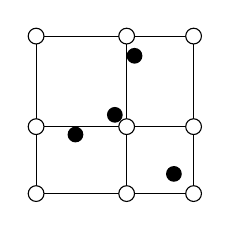
\begin{tikzpicture}
                \draw (0,0) rectangle (2.,2.);
                \draw (1.15,0.85) rectangle (2.,0);
                \draw (1.15,0.85) rectangle (2.,2);
                \draw (1.15,0.85) rectangle (0.,2);
                %% Old nodes
                \fill[white] (0,0) circle (0.1);
                \fill[white] (0,2) circle (0.1);
                \fill[white] (2,0) circle (0.1);
                \fill[white] (2,2) circle (0.1);
                \draw (0,0) circle (0.1);
                \draw (0,2) circle (0.1);
                \draw (2,0) circle (0.1);
                \draw (2,2) circle (0.1);
                
                %% Added nodes
                \fill[white] (1.15,0.85) circle (0.1);
                \fill[white] (0,0.85) circle (0.1);
                \fill[white] (2,0.85) circle (0.1);
                \fill[white] (1.15,0) circle (0.1);
                \fill[white] (1.15,2) circle (0.1);
                \draw (1.15,0.85) circle (0.1);
                \draw (0,0.85) circle (0.1);
                \draw (2,0.85) circle (0.1);
                \draw (1.15,0) circle (0.1);
                \draw (1.15,2) circle (0.1);
                
                %% Particles
                \fill[black] (0.5,0.75) circle (0.1); \fill[black] (1.25,1.75) circle (0.1); \fill[black] (1.75,0.25) circle (0.1); \fill[black] (1,1) circle (0.1);
              \end{tikzpicture}
            \end{column}
          \end{columns}
        \end{block}
      \end{column}
    \end{columns}
  \end{footnotesize}
\end{frame}
%%% Local Variables:
%%% mode: latex
%%% TeX-master: "../presentation"
%%% End:


%%% Local Variables:
%%% mode: latex
%%% TeX-master: "../presentation"
%%% End:
